\documentclass{standalone}
\usepackage{tikz}
\begin{document}
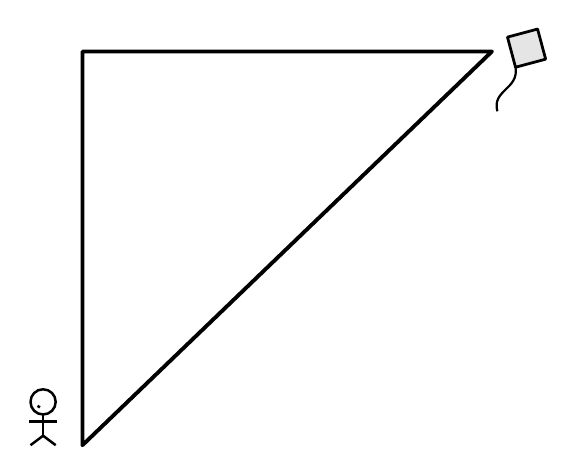
\begin{tikzpicture}[>=stealth, scale=1.0, line join=round]
  % Coordinates of the right triangle (kite problem)
  % Person stands at bottom-left corner (origin)
  % Vertical leg up the left side, horizontal leg across the top,
  % hypotenuse = kite string from person to kite at top-right.

  % Right triangle
  \draw[line width=1.4pt] (0,0) -- (0,5) -- (5.2,5) -- cycle;

  % Kite at the top-right end of the hypotenuse
  \begin{scope}[shift={(5.5,4.8)}, rotate=-30]
    \draw[line width=1pt, fill=black!10]
      (0,0) -- (0.28,0.28) -- (0,0.56) -- (-0.28,0.28) -- cycle;
    % kite tail
    \draw[line width=0.8pt] (0,0) .. controls (0.18,-0.22) and (-0.12,-0.4) .. (0.08,-0.6);
  \end{scope}

  % Stick figure (person) at the bottom-left
  \begin{scope}[shift={(-0.5,0)}, line width=0.9pt]
    \draw (0,0.55) circle (0.16);                 % head
    \draw (-0.07,0.50) -- (-0.04,0.48);           % (smile suggestion)
    \draw (0,0.39) -- (0,0.12);                    % body
    \draw (-0.18,0.30) -- (0.18,0.30);             % arms
    \draw (0,0.12) -- (-0.16,0) (0,0.12) -- (0.16,0); % legs
  \end{scope}
\end{tikzpicture}
\end{document}
